\section{GoogLeNet}
\label{googlenet}
GoogLeNet (in origine \textit{Inception v1}) è una rete neurale convoluzionale profonda presentata nel 2014 da Christian Szegedy, ricercatore presso Google, ed il suo team di ricerca. La pubblicazione del paper originale \cite{googlenet} è avvenuta poco dopo la schiacciante vittoria riportata da GoogLeNet nella \textit{ILSVRC 2014}\footnote{\url{http://image-net.org/challenges/LSVRC/2014/}}, sia nel problema di \textit{object classification} che in quello di \textit{object detection}, introdotto nell'anno precedente.

Il grande contributo di GoogLeNet nell'ambito  del deep learning è il miglioramento nell'utilizzo delle risorse computazionali da parte di una rete profonda, grazie all'introduzione del modulo \textit{Inception} (par. \ref{inception}. In particolare, se confrontata ad AlexNet (par. \ref{alexnet}), GoogLeNet utilizza circa 10 volte meno parametri (circa 6,8 milioni) essendo però significativamente più profonda (22 layer con parametri) e performante (errore \textit{top-5} su dataset ImageNet 6,7\%).\\

GoogLeNet è stata progettata per risolvere alcuni problemi tipici delle reti convoluzionali particolarmente profonde:

\begin{itemize}

\item L'operazione di convoluzione su volumi molto profondi è computazionalmente onerosa. Per risolvere questo problema, GoogLeNet introduce l'operazione di convoluzione $1\times 1$ (par. \ref{1x1conv}).

\item Le reti neurali molto profonde sono molto sensibili al rischio di \textit{overfitting}, a causa del loro alto grado di astrazione e rappresentazione dei concetti (dovuto al grandissimo numero di parametri). Questo problema è attenuato grazie all'introduzione della già citata operazione di convoluzione $1\times 1$, all'operazione di \textit{global average pooling} (par. \ref{globalAveragePooling}) e all'usuale pratica della \textit{image augmentation} (par. \ref{googlenetAugmentation}).

\item Le parti salienti di un'immagine possono avere delle dimensioni estremamente variabili all'interno di essa. Si guardi ad esempio la figura seguente: 

\begin{figure}[h!] 
\centering
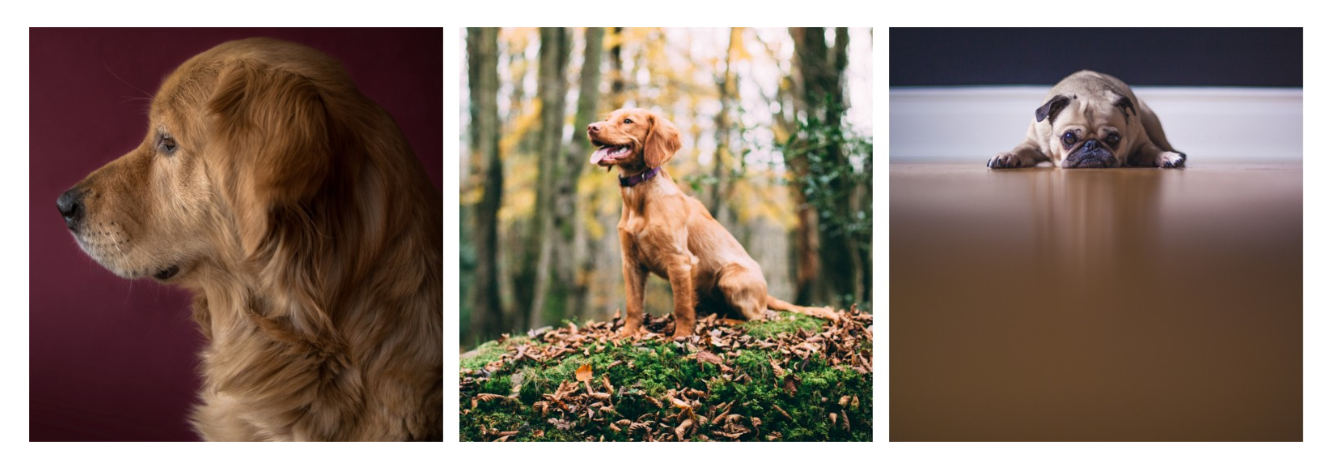
\includegraphics[width=0.9\textwidth]{cani.png}
\caption{Tre immagini di cani. L'area occupata da ciascun cane è differente e via via più piccola in ogni immagine}
\label{fig:cani}
\end{figure}

A causa di questa grande variabilità nella localizzazione dell'informazione la scelta delle dimensioni dei filtri convoluzionali diventa complessa. Un filtro più ampio è preferito quando l'informazione è distribuita su un'area vasta dell'immagine; un filtro più piccolo è adeguato in quei casi in cui l'informazione è localizzata in un'area più ristretta.\\
Questo problema è risolto con l'introduzione dei moduli \textit{inception} (par. \ref{inception}).

\item A causa della profondità di una rete, un altro tipico problema che si presenta durante l'addestramento è la scomparsa del gradiente (\textit{vanishing gradient problem}, par. \ref{vanishingGradient}), nella fase di \textit{backpropagation}. Questo problema è risolto prevedendo una particolare architettura della rete, che in fase di addestramento risulta in realtà composta da tre sottoreti diverse (par. \ref{classificatoriAusiliari}).

\end{itemize}


\subsection{Convoluzione $1\times 1$}
\label{1x1conv}
Mutuando un'idea precedentemente esposta in \cite{NiN}, GoogLeNet introduce l'operazione di convoluzione $1\times 1$ (seguita dalla funzione di attivazione ReLU). Lo scopo di questa operazione è quello di ridurre le dimensioni (in particolare, la profondità) di un volume di attivazioni per ridurre il costo computazionale delle operazioni di convoluzione successive. Questo permette di ottenere reti più profonde ma anche - con il modulo \textit{inception} (par. \ref{inception}) - più "larghe".
La fig. \ref{fig:1x1conv} mostra schematicamente l'applicazione di un'operazione di convoluzione $1\times 1$.

\begin{figure}[h] 
\centering
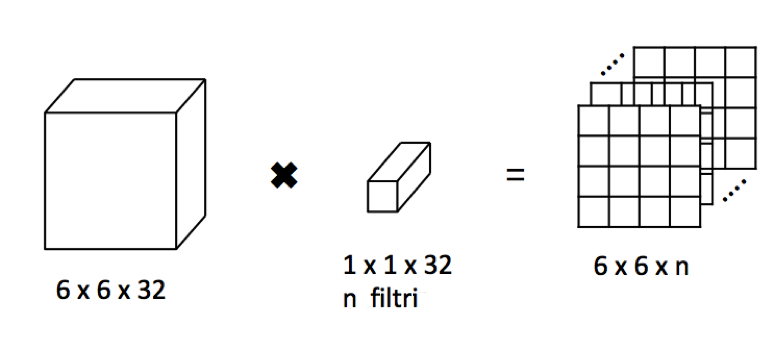
\includegraphics[width=0.85\textwidth]{1x1conv.png}
\caption{Convoluzione $1\times 1$ applicata ad un volume di attivazioni $6\times 6\times 32$. La profondità del volume di output dipende dal n. di filtri $1\times 1$ adoperati. In questo caso si ottiene una riduzione della profondità per $n<32$.}
\label{fig:1x1conv}
\end{figure}

Grazie all'introduzione della convoluzione $1\times 1$, inoltre, il numero di pesi nei kernel delle operazioni di convoluzione successive diminuiscono, riducendo così il rischio di overfitting.\\

A conclusione del paragrafo viene riportata un'osservazione interessante. Le reti neurali artificiali "standard" (contenenti cioè solo strati completamente connessi) possono essere convertite in reti convoluzionali mediante sole convoluzioni $1\times 1$. Infatti nelle ANN con soli strati completamente connessi tutti i volumi su cui si opera hanno dimensione $1\times 1\times k$, dove $k$ è variabile ed è il numero $k$ di neuroni dello strato che ha generato tale volume; si può allora pensare a ciascuno di questi strati completamente connessi con $k$ neuroni (biunivocamente associati al volume che generano in output) come ad uno strato di convoluzione $1\times 1$ che applica $k$ filtri al volume in input. Ogni neurone del volume di output $1\times 1\times n$ ha così una completa connettività con tutti i neuroni del volume (e quindi dello strato completamente connesso) precedente.

\subsection{Modulo \textit{Inception}}
\label{inception}
Per ovviare al problema della variabilità dell'area occupata da un oggetto da classificare in un'immagine, l'idea chiave è stata quella di operare molteplici convoluzioni, con diverse dimensioni dei kernel, in parallelo.
Così facendo la rete tende a diventare più "larga" anziché più "profonda".
Il modulo \textit{inception} è stato sviluppato proprio sulla base di questa idea.
In fig. \ref{fig:inception} è mostrato il modulo \textit{inception}, innestato più volte nell'architettura di GoogLeNet (par. \ref{architetturaGooglenet})

\begin{figure}[h] 
\centering
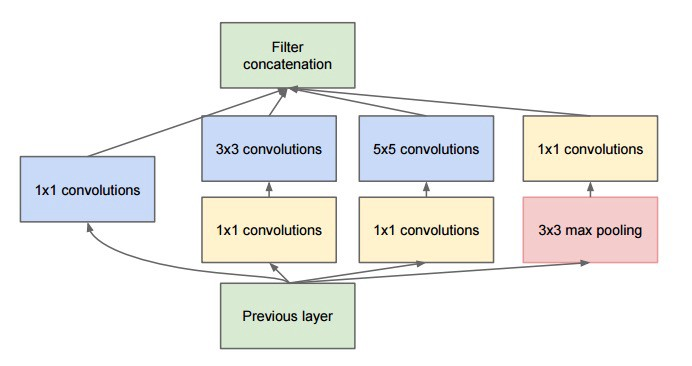
\includegraphics[width=\textwidth]{inception.jpg}
\caption{Modulo \textit{inception}}
\label{fig:inception}
\end{figure}

Tale modulo riceve un volume di input da uno strato precedente e opera in parallelo su di esso tre convoluzioni (con filtri $1\times 1$, $3\times 3$, $5\times 5$ rispettivamente) e un \textit{max pooling} con finestra $3\times 3$. Per diminuire il costo computazionale delle operazioni di convoluzione, si è deciso di implementare una convoluzione $1\times 1$ prima delle convoluzioni $3\times 3$ e $5\times 5$ e dopo il \textit{max pooling} $3\times 3$.
Gli output sono infine "impilati" tra loro lungo la dimensione della profondità, e il volume risultante viene inviato al successivo layer(o modulo \textit{inception}).

\subsection{Classificatori ausiliari}
\label{classificatoriAusiliari}
L'architettura di GoogLeNet prevede, per la sola fase di addestramento, delle "diramazioni", posizionate circa a metà della rete, evidenti in fig. \ref{architetturaGooglenet}.
Questi rami della rete ospitano dei classificatori ausiliari che consistono di
\begin{itemize}
\item Average Pooling $5\times 5$ (Stride 3)
\item Convoluzione $1\times 1$ (128 filtri)
\item ReLU layer
\item 1024 Fully Connected layer
\item 1000 Fully Connected layer
\item Dropout layer (70\% di probabilità di dropout di ciascun output; vd. par. \ref{dropout})
\item Softmax layer
\end{itemize}
Questa particolare architettura è stata ideata per attenuare il problema della scomparsa del gradiente (\textit{vanishing gradient problem}, par. \ref{vanishingGradient}), tipico delle reti molto profonde. L'idea si basa su un'osservazione: le promettenti performance di reti meno profonde nei task di \textit{image classification} suggeriscono che le \textit{feature} estratte dagli strati intermedi della rete hanno un grande impatto sulla predizione finale. Pertanto, nel tentativo di propagare meglio il segnale gradiente all'indietro (cioè per amplificarlo), la funzione costo calcolata è amplificata sulla base delle predizioni dei classificatori intermedi.
In fase di addestramento, dai valori di output dello strato softmax dei tre classificatori (i due intermedi e quello finale) viene calcolata la funzione costo (\textit{cross-entropy loss}). 
Il costo totale sarà costituito dalla somma pesata del costo registrato dal classificatore finale (con peso 1) e quello registrato dai due classificatori ausiliari (con peso $0.3$).

\subsection{Global Average Pooling}
\label{globalAveragePooling}
In precedenza, nella parte conclusiva delle architetture delle reti convoluzionali venivano posti due o più layer completamente connessi (ad esempio in AlexNet, par. \ref{alexnet}, che presenta tre fully connected layer finali).
Mutuando un'idea esposta in \cite{NiN}, in GoogLeNet si è previsto invece un singolo layer completamente connesso finale con 1000 neuroni (quello che fornisce valori alla funzione softmax) preceduto da uno strato di pooling denominato \textit{global average pooling}. Questo strato opera un pooling su una superficie $7\times 7$ (le dimensioni di base e altezza del volume di output precedente) e restituisce una superficie $1\times 1$, il cui valore è la media calcolata sui 49 valori dei neuroni della superficie. Gli autori hanno mostrato che passare da un fully connected layer a un average pooling layer ha contribuito a migliorare la \textit{top-1 accuracy} nella ILSVRC del 0.6\%, abbassando ulteriormente il numero dei pesi della rete (da circa 51.2 milioni se fosse stato utilizzato il FC layer agli 0 del global average pooling). In questo modo, GoogLeNet è stata resa anche leggermente più robusta all'\textit{overfitting}.
La fig. \ref{fig:FCvsGAP} mostra un confronto tra il funzionamento di un FC layer e un GAP (Global Average Pooling) layer.

\begin{figure}[h]
\centering
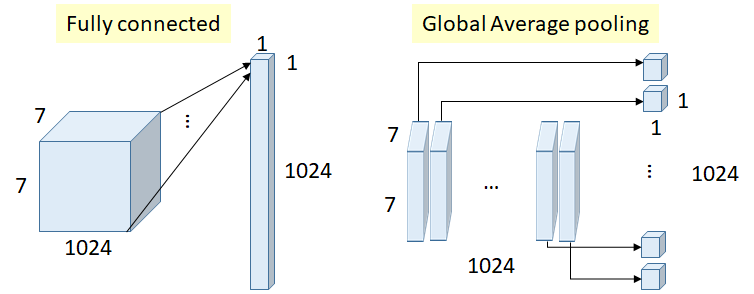
\includegraphics[width=0.85\textwidth]{FCvsGAP.png}
\caption{Confronto fra un FC layer e un GAP layer}
\label{fig:FCvsGAP}
\end{figure}

\subsection{Data Augmentation}
\label{googlenetAugmentation}
Per ridurre ulteriormente l'overfitting al training set di ImageNet, GoogLeNet fa uso di una particolare tecnica di \textit{data augmentation} (par. \ref{augmentation}). Al posto delle immagini originali, per l'addestramento sono stati utilizzati dei ritagli (uno per ciascuna immagine di un mini-batch) di dimensioni distribuite uniformemente tra l'8\% e il 100\% dell'intera immagine e con \textit{aspect ratio} (rapporto tra larghezza e altezza dell'immagine) distribuito uniformemente tra 3/4 e 4/3. In aggiunta, sono state operate alcune distorsioni fotometriche già adoperate in precedenza in \cite{photometric}.

\subsection{Architettura di GoogLeNet}
\label{architetturaGooglenet}
L'architettura di GoogLeNet è riportata in forma tabellare in tab. \ref{tab:tabellaGooglenet} e in forma grafica in fig. \ref{fig:googlenet}

\begin{figure}[h]
\centering
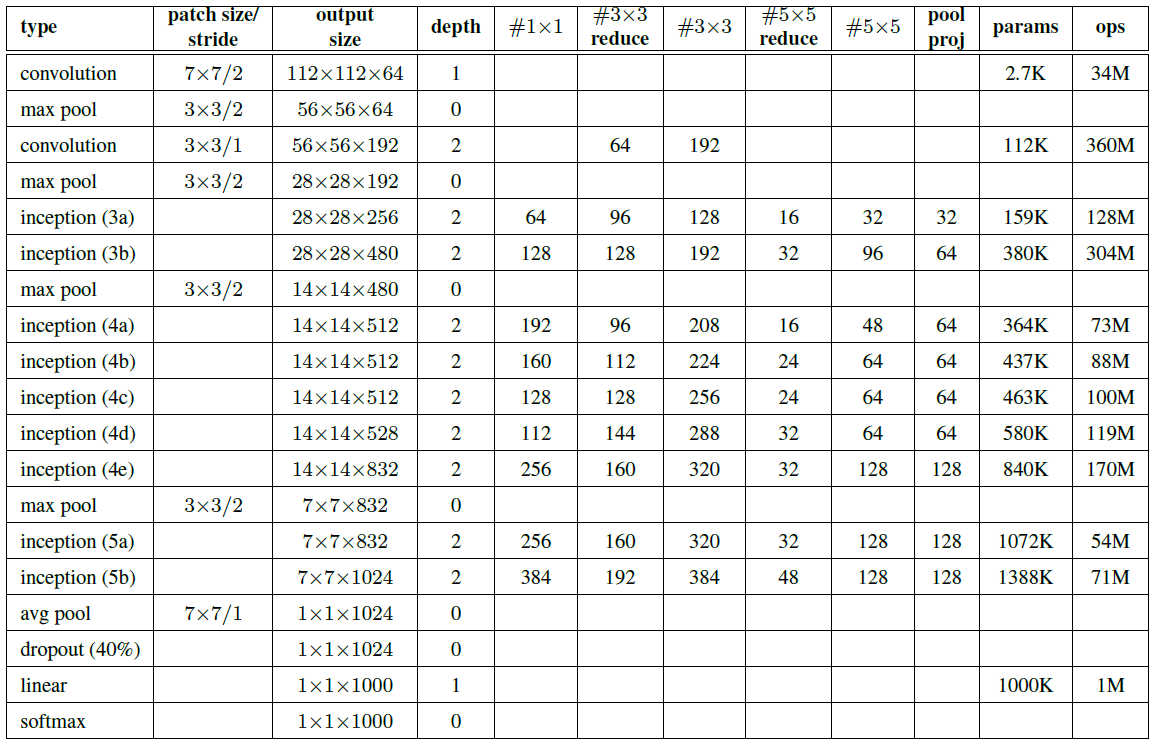
\includegraphics[width=0.9\textwidth]{tabellaGooglenet.png}
\caption{Architettura di GoogLeNet}
\label{tab:tabellaGooglenet}
\end{figure}

\begin{figure}[tb] 
\centering
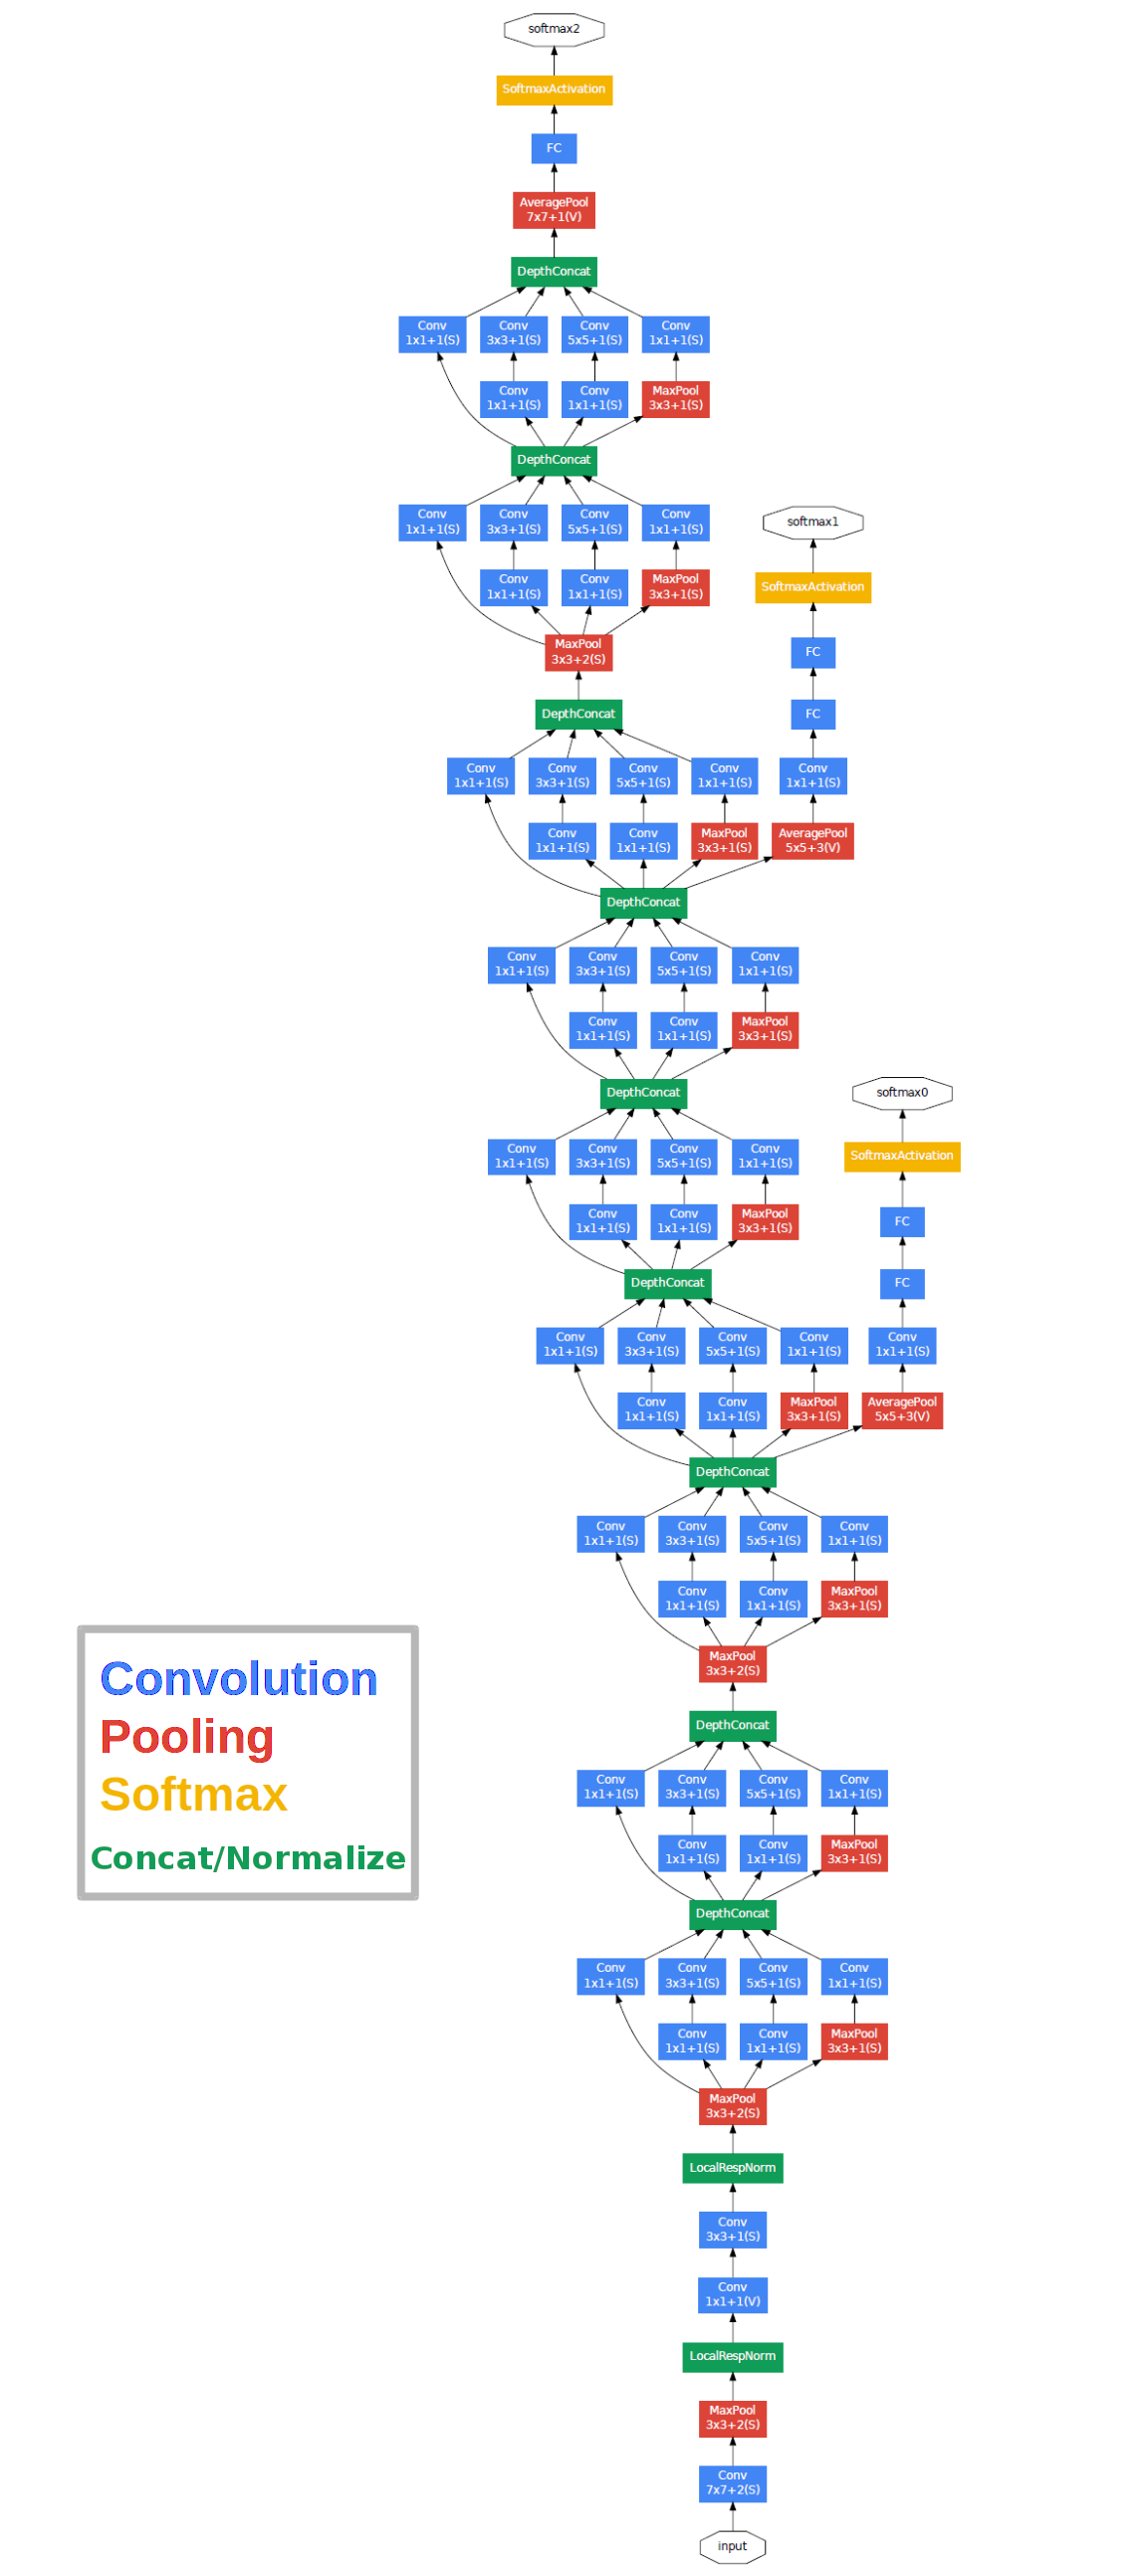
\includegraphics[width=0.95\textwidth, height=0.99\textheight, keepaspectratio]{GoogLeNet.png}
\caption{Architettura di GoogLeNet}
\label{fig:googlenet}
\end{figure}

La rete accetta in input immagini $224\times 224$. I primi layer parametrizzati dall'inizio della rete sono 3 layer convoluzionali, a cui seguono 9 moduli \textit{inception} (ognuno con 6 layer convoluzionali) e infine un fully connected layer (finale).
Si evidenzia nuovamente, come già esposto nel par. \ref{classificatoriAusiliari}, che le ramificazioni che ospitano i due classificatori ausiliari esistono solo in fase di addestramento, e vengono eliminati dopo di esso.

\subsection{Addestramento di GoogLeNet}
GoogLeNet fu addestrato sul dataset di ImageNet (par. \ref{imagenet}) su una macchina che usava solamente le sue CPU per effettuare calcoli\footnote{Tuttavia gli autori affermano che se fosse stato usato un ridotto numero di GPU di fascia alta l'addestramento avrebbe potuto essere effettuato in meno di una settimana (avendo come unica limitazione la memoria delle GPU stesse).}, usando come algoritmo di ottimizzazione la discesa stocastica del gradiente con momento = 0.9, \textit{learning rate}\footnote{Per la ILSVRC 2014, il team ha in realtà utilizzato un ensemble di 7 reti GoogLeNet diverse, ognuna addestrata con \textit{learning rate} iniziale e \textit{mini-batch size} diversi} con \textit{annealing} del 4\% ogni 8 epoche. Dettagli più specifici sulla fase di addestramento di GoogLeNet possono essere trovati nel paper originale \cite{googlenet}.